\documentclass[12pt]{article}

% Packages
\usepackage[utf8]{inputenc}
\usepackage{amsmath, amssymb}
\usepackage{algorithmic}
\usepackage{fancyhdr}
\usepackage{geometry}
\usepackage{booktabs}
\usepackage{array}
\usepackage{hyperref}
\usepackage{graphicx}
\usepackage{amsthm}
\usepackage{forest}

% Page setup
\geometry{margin=1in}
\pagestyle{fancy}
\fancyhf{}
\rhead{CSCE 608 --- Spring 2026}
\lhead{Darwin White}
\cfoot{\thepage}

% Title
\title{Project 1 Report}
\author{CSCE 608 \\ Dr. Jianer Chen \\ Spring 2026 \\ \vspace{0.5cm} \textbf{Darwin White, 231007562}}
\date{}

\begin{document}
\maketitle
\thispagestyle{fancy}

\section*{Website and Source Code}

Website: \href{https://csce608-project.onrender.com/}{https://csce608-project.onrender.com/}\\
Source code: \href{https://github.com/DarwinWhite/csce608_project}{https://github.com/DarwinWhite/csce608\_project}\\
\textbf{NOTE:} Upon trying to load the actual website there will be about a 60-90 second spin up time due to the free tier of Render.

\section*{Project Description}

I propose a database application that follows project idea $13$ from the sample topics. My database application will implement an Art Gallery Management Database which models the artists, artwork, customers, and staff of the art gallery itself. I will break these entities down into the following attributes.

\begin{enumerate}
    \item Artists with attributes: \underline{artistID}, name, style, medium
    \item Artwork with attributes: \underline{artworkID}, artist, title, yearMade, style, price, isSold
    \item Customers with attributes: \underline{customerID}, name, phoneNum, email, moneySpent
    \item Staff with  attributes: \underline{staffID}, name, phoneNum, role
    \item Gallery with attributes: \underline{galleryID}, name, address, openHours
\end{enumerate}

This database construction can be used to manage one specific Gallery or many Galleries if the application requires it. For the application itself, I will be making a simple three page construction that has a user interface, a staff interface, and a management interface. The user interface will allow users to query artists and artwork in search of specific pieces. This will involve simple select statements and joins. For the staff and management interfaces, I will incorporate more data analytics using more complex SQL queries to determine sales over time, specific artist sales, customer preferences, and more. The management interface will also specifically contain procedures and SQL queries to edit the management database like addding or removing staff, art, or artists.

I anticipate the most difficult portion will be creating the complex SQL queries for the data analytics on the staff interface. These may require complex joins or nested subqueries. However, I will be building a script to create the data I need for the database, so I will create the data in such a way that the data for the analytics should already exist. I.e., I will include data over a time period of three years, as well as include a large quantity of customers and artwork to support the sales data I plan on creating. All that will be required is to create queries that grab the information correctly.

The majority of this project will be done in Python, using a FastAPI web application that simply exposes the endpoints to a dummy front end that simply has tables and graphs for the user. The data collection script will also be in Python. The database itself will be a postgres database running a Docker container, with the whole app containerized together with Docker compose. This should ensure easy hosting on Heroku as well as easy setup and tear down.

\newpage

\section*{E/R Diagram}

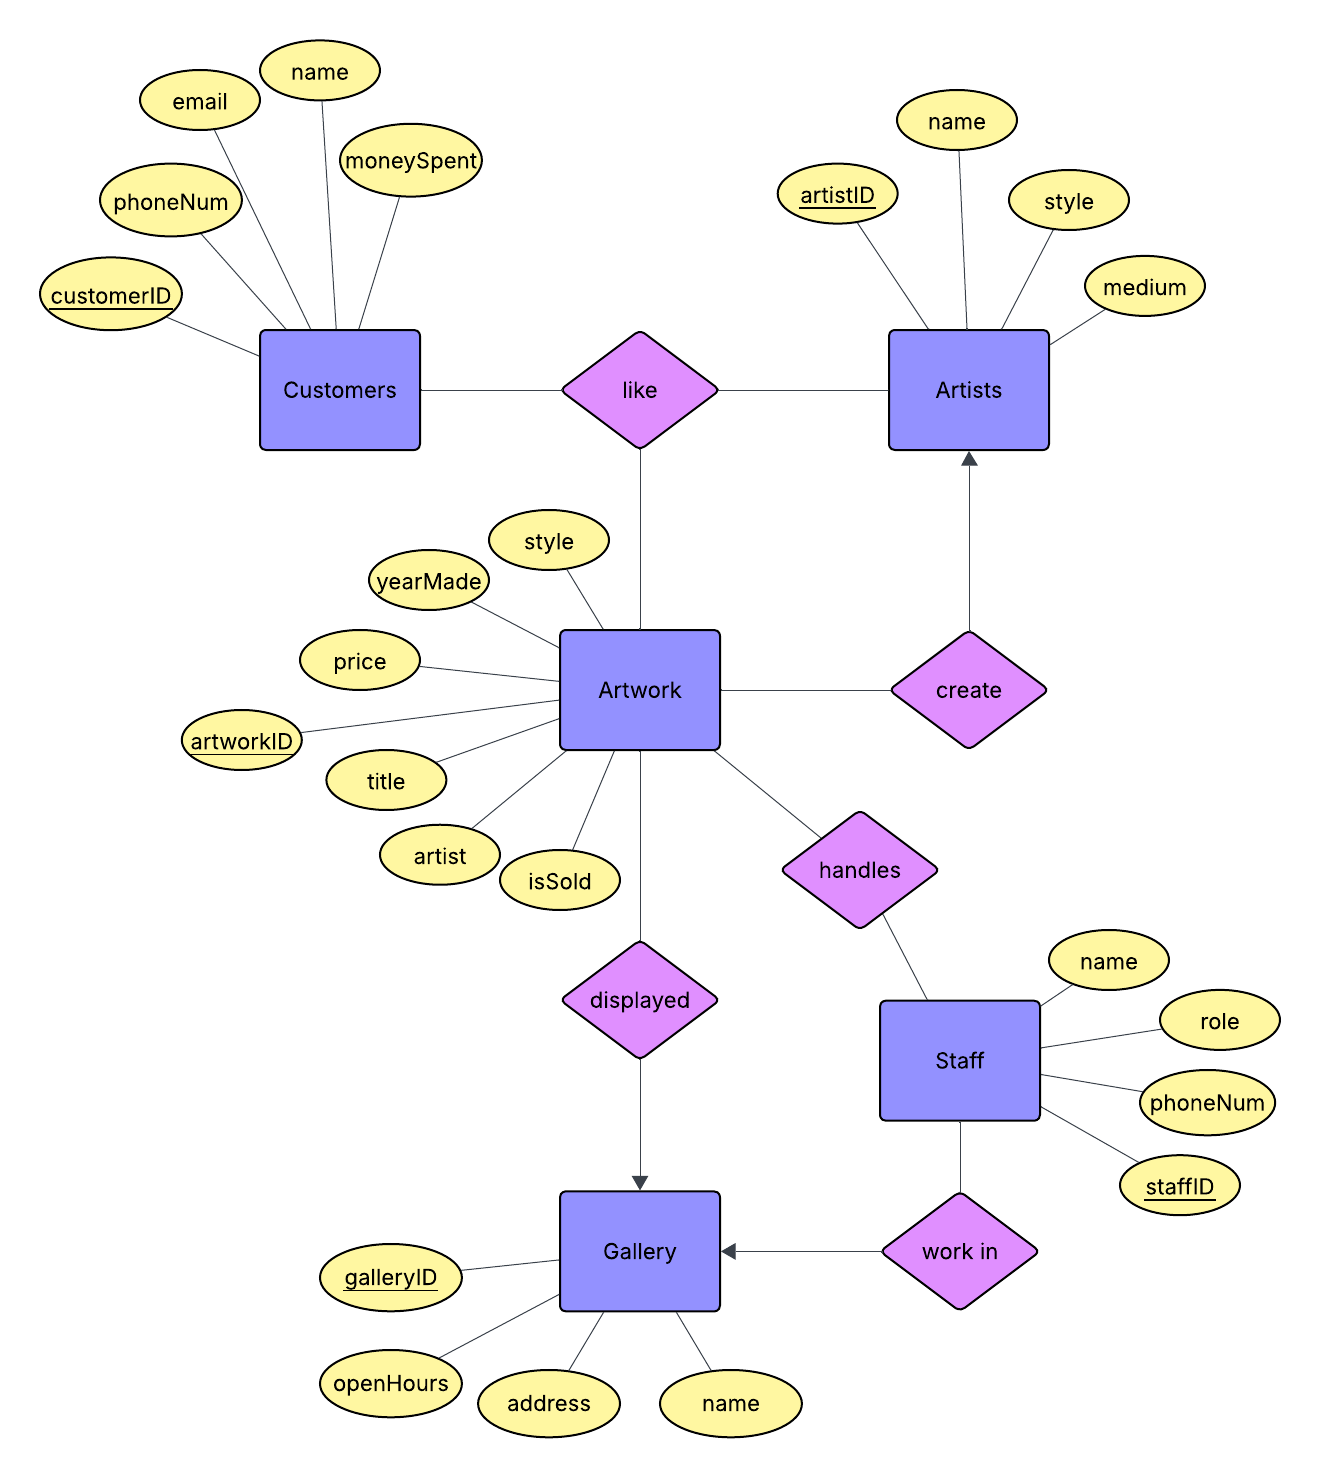
\includegraphics[width=\textwidth]{CSCE_608_Project_1_ER.png}

\newpage

\section*{Relational Schema}

1. The Relational Schema would be as presented below. Note: given the many-to-one constraints in the ER diagram, relationship sets Create, Displayed, and WorkIn were not converted into separate relations. Instead, their corresponding foreign keys were incorporated into the Artwork and Staff relations. This avoids redundancy and reflects the functional dependencies implied by the constraints (e.g., artworkID → artistID and artworkID → galleryID). \\

Customers(\underline{customerID}, name, phoneNum, email, moneySpent)

Artists(\underline{artistID}, name, style, medium)

Artwork(\underline{artworkID}, title, yearMade, style, price, isSold, artistID, galleryID)

Staff(\underline{staffID}, name, phoneNum, role, galleryID)

Gallery(\underline{galleryID}, name, address, openHours)

Like(\underline{customerID}, \underline{artworkID}, \underline{artistID})

Handles(\underline{staffID}, \underline{artworkID}) \\

\noindent 2. All the nontrivial functional dependencies are:

(customerID $\rightarrow$ name, phoneNum, email, moneySpent)

(artistID $\rightarrow$ name, style, medium)

(artworkID $\rightarrow$ title, yearMade, style, price, isSold, artistID, galleryID)

(staffID $\rightarrow$ name, phoneNum, role, galleryID)

(galleryID $\rightarrow$ name, address, openHours)\\ 

\noindent 3. We examine each relation in the schema to determine whether it satisfies Boyce-Codd Normal Form (BCNF). A relation is in BCNF if, for every nontrivial functional dependency $X \rightarrow Y$, $X$ is a superkey.

\subsection*{Customers}
Relation: Customers(\underline{customerID}, name, phoneNum, email, moneySpent)

Functional Dependency:
\[
(\text{\underline{customerID}} \rightarrow \text{name, phoneNum, email, moneySpent})
\]

Since \underline{customerID} is the primary key, it is a superkey. Therefore, the relation satisfies BCNF.

\subsection*{Artists}
Relation: Artists(\underline{artistID}, name, style, medium)

Functional Dependency:
\[
(\text{\underline{artistID}} \rightarrow \text{name, style, medium})
\]

Since \underline{artistID} is the primary key, the relation satisfies BCNF.

\subsection*{Gallery}
Relation: Gallery(\underline{galleryID}, name, address, openHours)

Functional Dependency:
\[
(\text{\underline{galleryID}} \rightarrow \text{name, address, openHours})
\]

Since \underline{galleryID} is the primary key, the relation satisfies BCNF.

\subsection*{Artwork}
Relation: Artwork(\underline{artworkID}, title, yearMade, style, price, isSold, artistID, galleryID)

Functional Dependency:
\[
(\text{\underline{artworkID}} \rightarrow \text{title, yearMade, style, price, isSold, artistID, galleryID})
\]

This dependency arises from the assumption that each artwork is created by exactly one artist and displayed in exactly one gallery. Since \underline{artworkID} is the primary key, it is a superkey, and the relation satisfies BCNF.

\subsection*{Staff}
Relation: Staff(\underline{staffID}, name, phoneNum, role, galleryID)

Functional Dependency:
\[
(\text{\underline{staffID}} \rightarrow \text{name, phoneNum, role, galleryID})
\]

This dependency arises from the assumption that each staff member works in exactly one gallery. Since \underline{staffID} is the primary key, the relation satisfies BCNF.

\subsection*{Like}
Relation: Like(\underline{customerID}, \underline{artistID}, \underline{artworkID})

There are no nontrivial functional dependencies in this relation. Therefore, it trivially satisfies BCNF.

\subsection*{Handles}
Relation: Handles(\underline{staffID}, \underline{artworkID})

There are no nontrivial functional dependencies in this relation. Therefore, it trivially satisfies BCNF. \\

All relations in the schema satisfy the BCNF condition. For each nontrivial functional dependency, the left-hand side is a superkey. Additionally, relations with no nontrivial functional dependencies trivially satisfy BCNF. Therefore, no decomposition was necessary, and the schema is free of redundancy caused by functional dependencies.

\newpage

\section*{Data Collection}

All data in the system is synthetically generated using a Python script that leverages the \texttt{Faker} library alongside curated vocabulary lists. Faker is used to produce realistic values for attributes such as customer names, phone numbers, and email addresses, while artist names are similarly generated to resemble real people. For attributes that require domain-specific vocabulary, such as artistic style and medium, I constructed explicit lists of valid values (e.g., Impressionism, Abstract, Oil on canvas, Watercolor) and sampled from them at random. Artwork titles are procedurally constructed by combining adjectives and subjects drawn from curated word lists, yielding titles such as ``Luminous Shore at Dusk'' or ``Forgotten Elegy in Blue.'' Artwork prices follow a log-uniform distribution between \$500 and \$500{,}000, which produces a realistic spread of inexpensive and high-value pieces rather than a flat uniform distribution. Roughly 40\% of all artwork is marked as sold, and for each sold piece a random customer is selected as the buyer and their \texttt{moneySpent} attribute is incremented accordingly.

Uniqueness of key attributes is enforced at two levels. At the database level, all primary keys use the \texttt{SERIAL} type, which guarantees auto-incremented unique integers with no application-level intervention required. The \texttt{email} column in the \texttt{Customers} table carries a \texttt{UNIQUE} constraint, so duplicate emails are rejected by the database even if the seed script were to produce a collision. For composite-key relations, uniqueness is enforced in the seed script itself: Python \texttt{set} objects track already-inserted \texttt{(customerID, artworkID)} pairs for the \texttt{Like} relation and \texttt{(staffID, artworkID)} pairs for the \texttt{Handles} relation, skipping any pair that would produce a duplicate before attempting an insert. Additionally, the \texttt{artistID} stored in each \texttt{Like} row is always set equal to the \texttt{artistID} of the referenced artwork, ensuring referential consistency and enabling direct joins between \texttt{Like} and \texttt{Artists} without needing to traverse \texttt{Artwork} as an intermediary.

\newpage

\section*{User Interface}

The user interface consists of three separate web pages served by the FastAPI backend: a visitor page, a staff page, and a management page. The visitor page allows any user to browse the gallery's artwork and artists using filter controls for style, price range, and availability, and to view four Chart.js data visualizations. The staff page allows a staff member to select themselves from a dropdown and manage their assigned artwork, mark pieces as sold, add new pieces to the gallery, and search customer records. The management page provides full create, read, update, and delete functionality for all entities through a tabbed layout, as well as a dedicated analytics tab with six charts covering revenue, customer spending, artist popularity, and staff assignments. All data access is implemented using raw SQL through the psycopg2 library. The system offers the following key functions:

\begin{enumerate}
    \item \textbf{Gallery information retrieval} --- A simple \texttt{SELECT} fetches the single gallery record to populate the page header. This is the most basic query in the system: \texttt{SELECT * FROM Gallery LIMIT 1}.

    \item \textbf{Filtered artwork browsing with pagination} --- Users may filter artwork by style, price range, sold status, and artist. The query is dynamically constructed with optional \texttt{WHERE} clauses and uses an inner \texttt{JOIN} to include each artwork's artist name in a single round trip: \texttt{SELECT aw.*, ar.name FROM Artwork aw JOIN Artists ar ON ar.artistID = aw.artistID WHERE aw.style = \%s AND aw.price >= \%s ORDER BY aw.artworkID LIMIT \%s OFFSET \%s}.

    \item \textbf{Artist listing with artwork count} --- A \texttt{LEFT JOIN} with \texttt{GROUP BY} aggregation retrieves each artist alongside the number of pieces they have in the gallery. A \texttt{LEFT JOIN} is used rather than an inner join so that artists with no artwork still appear: \texttt{SELECT a.*, COUNT(aw.artworkID) AS artwork\_count FROM Artists a LEFT JOIN Artwork aw ON aw.artistID = a.artistID GROUP BY a.artistID ORDER BY a.name}.

    \item \textbf{Artwork count by style} --- A straightforward aggregation query powers the bar chart on the visitor page, requiring no joins: \texttt{SELECT style, COUNT(*) AS count FROM Artwork GROUP BY style ORDER BY count DESC}.

    \item \textbf{Revenue by style} --- This query filters for sold artwork only and aggregates total revenue and piece count per style, combining a conditional \texttt{WHERE} clause with \texttt{SUM} and \texttt{GROUP BY}: \texttt{SELECT style, SUM(price) AS total\_revenue, COUNT(*) AS sold\_count FROM Artwork WHERE isSold = TRUE GROUP BY style ORDER BY total\_revenue DESC}.

    \item \textbf{Most liked artists} --- The most complex analytics query joins the \texttt{Like} relation directly to the \texttt{Artists} relation and counts likes per artist. Because \texttt{artistID} is stored in \texttt{Like}, no intermediate join through \texttt{Artwork} is needed, which demonstrates the utility of the schema design decision to carry that foreign key: \texttt{SELECT ar.name, COUNT(l.artworkID) AS like\_count FROM "Like" l JOIN Artists ar ON ar.artistID = l.artistID GROUP BY ar.artistID, ar.name ORDER BY like\_count DESC LIMIT 10}.
\end{enumerate}

\newpage

\section*{Discussion}

The most significant technical difficulty I encountered was in deploying the application to a hosted environment. Initially, the database seed script was called synchronously during application startup, which caused the server to block for several minutes before it could respond to any requests. On Render's free hosting tier, this caused the deployment health check to time out and the service to repeatedly fail to start. I resolved this by moving the seed call into a background thread, allowing the server to become responsive immediately while seeding continued in the background. A related issue was that the schema had originally been applied only through Docker's \texttt{docker-entrypoint-initdb.d} mechanism, which does not execute when the application connects to an external managed database such as the one provided by Render. This required adding a programmatic schema application step at startup that reads the \texttt{schema.sql} file and executes it through psycopg2 directly, using \texttt{IF NOT EXISTS} guards throughout to ensure the operation is safe to run on every startup.

From a database perspective, the most instructive aspect of the project was designing and implementing the analytics queries. Writing aggregations that span multiple relations, such as computing total revenue broken down by artistic style or ranking artists by the number of customer likes, required careful thought about join ordering and the correct placement of \texttt{WHERE} clauses relative to \texttt{GROUP BY}. I also gained a greater appreciation for how early schema decisions propagate through the rest of a project. Storing \texttt{artistID} directly in the \texttt{Like} relation, for example, simplified several analytics queries and eliminated unnecessary joins, while still conforming to the given relational schema. Overall, this project reinforced that well-considered schema design and precise SQL are far more impactful than application-layer complexity when building a data-driven system.

\end{document}